% This is a Basic Assignment Paper but with like Code and stuff allowed in it, there is also url, hyperlinks from contents included. 

\documentclass[11pt]{article}

% Preamble

\usepackage[margin=1in]{geometry}
\usepackage{amsfonts, amsmath, amssymb}
\usepackage{fancyhdr, float, graphicx}
\usepackage[utf8]{inputenc} % Required for inputting international characters
\usepackage[T1]{fontenc} % Output font encoding for international characters
\usepackage{fouriernc} % Use the New Century Schoolbook font
\usepackage[nottoc, notlot, notlof]{tocbibind}
\usepackage{listings}
\usepackage{xcolor}
\usepackage{blindtext}
\usepackage{hyperref}
\hypersetup{
    colorlinks=true,
    linkcolor=black,
    filecolor=magenta,      
    urlcolor=cyan,
    pdfpagemode=FullScreen,
    }

\definecolor{codegreen}{rgb}{0,0.6,0}
\definecolor{codegray}{rgb}{0.5,0.5,0.5}
\definecolor{codepurple}{rgb}{0.58,0,0.82}
\definecolor{backcolour}{rgb}{0.95,0.95,0.92}

\lstdefinestyle{mystyle}{
    backgroundcolor=\color{backcolour},   
    commentstyle=\color{codegreen},
    keywordstyle=\color{magenta},
    numberstyle=\tiny\color{codegray},
    stringstyle=\color{codepurple},
    basicstyle=\ttfamily\footnotesize,
    breakatwhitespace=false,         
    breaklines=true,                 
    captionpos=b,                    
    keepspaces=true,                 
    numbers=left,                    
    numbersep=5pt,                  
    showspaces=false,                
    showstringspaces=false,
    showtabs=false,                  
    tabsize=2
}

\lstset{style=mystyle}

% Header and Footer
\pagestyle{fancy}
\fancyhead{}
\fancyfoot{}
\fancyhead[L]{\textit{\Large{Internet of Things Lab Assignment 3}}}
\fancyhead[R]{\textit{\Large{Krishnaraj}}}
\fancyfoot[C]{\thepage}
\renewcommand{\footrulewidth}{1pt}



% Other Doc Editing
% \parindent 0ex
%\renewcommand{\baselinestretch}{1.5}

\begin{document}

\begin{titlepage}
	\centering

	%---------------------------NAMES-------------------------------

	\huge\textsc{
		MIT World Peace University
	}\\

	\vspace{0.75\baselineskip} % space after Uni Name

	\LARGE{
		Internet of Things\\
		Second Year B. Tech, Semester 2
	}

	\vfill % space after Sub Name

	%--------------------------TITLE-------------------------------

	\rule{\textwidth}{1.6pt}\vspace*{-\baselineskip}\vspace*{2pt}
	\rule{\textwidth}{0.6pt}
	\vspace{0.75\baselineskip} % Whitespace above the title



	\huge{\textsc{
			Interface of Servo Motor like Actuators with Development Boards
		}} \\



	\vspace{0.5\baselineskip} % Whitespace below the title
	\rule{\textwidth}{0.6pt}\vspace*{-\baselineskip}\vspace*{2.8pt}
	\rule{\textwidth}{1.6pt}

	\vspace{1\baselineskip} % Whitespace after the title block

	%--------------------------SUBTITLE --------------------------	

	\LARGE\textsc{
		Assignment 3
	} % Subtitle or further description
	\vfill

	%--------------------------AUTHOR-------------------------------

	Prepared By
	\vspace{0.5\baselineskip} % Whitespace before the editors

	\Large{
		Krishnaraj Thadesar \\
		Cyber Security and Forensics\\
		Batch A2, PA 20
	}


	\vspace{0.5\baselineskip} % Whitespace below the editor list
	\today

\end{titlepage}


\tableofcontents
\thispagestyle{empty}
\clearpage

\setcounter{page}{1}

\section{Aim}
To interface simple actuators such as DC Motor with Raspberry Pi/ ESP8266 boards / Beagle bone board/ Tinker CAD Arduino Uno.

\section{Objectives}
\begin{itemize}
	\item To understand actuators interfacing with development boards
	\item Servo Motor control using LN298 motor driver and Arduino Uno
\end{itemize}

\section{Component List}
\begin{table}[H]
	\begin{tabular}{|c|c|c|}
		\hline
		\textbf{Name} & \textbf{Quantity} & \textbf{Component}         \\ \hline
		U1            & 1                 & Arduino Uno R3             \\ \hline
		DIST1         & 1                 & Ultrasonic Distance Sensor \\ \hline
		SERVO1        & 1                 & Positional Micro Servo     \\ \hline
	\end{tabular}
\end{table}
\section{Theory}
\subsection{Stepper Motor}

A stepper motor is a type of electric motor that rotates in small,
precise steps. Stepper motors are commonly used in applications that
require precise positioning, such as robotics, CNC machines, and 3D
printers. Stepper motors have multiple coils that are energized in a
specific sequence to produce precise steps of rotation.\\

The rotation of the stepper motor is controlled by a series of pulses sent to the motor
driver, which energizes the coils in the correct sequence.

\subsection{DC Motor}

A DC (direct current) motor is a type of electric motor that uses a
magnetic field to produce rotational motion. DC motors typically have
two terminals that are connected to a DC power source. \\

When a
current is applied to the motor, it generates a magnetic field that
interacts with the magnetic field of the stator, causing the rotor to
rotate. DC motors are commonly used in applications that require high
torque and low speed, such as robotics, conveyor systems, and electric
vehicles.

\subsection{Servo Motor}
A servo motor is a type of electric motor that uses feedback to control
the position of the output shaft. Servo motors are commonly used in
applications that require precise control of position and speed, such as
robotics, RC cars, and model airplanes.\\

Servo motors have a built-in
feedback mechanism that detects the position of the output shaft and
adjusts the motor's operation accordingly. Servo motors typically have
a limited range of motion (usually less than 180 degrees) and are used
for applications that require precise control of motion.


\subsection{LN298 Motor Driver}
\begin{enumerate}
	\item Dual H-bridge configuration: The L298 consists of two H-bridge circuits,
	      which allows it to drive two DC motors or one bipolar stepper motor.
	\item High current capacity: The L298 can handle a maximum current of up to 2
	      amps per channel, which makes it suitable for driving high-power motors.
	\item Low voltage drop: The L298 has a low voltage drop, which means that it
	      can operate with low voltage power supplies.
	\item Built-in protection features: The L298 includes built-in protection features
	      such as thermal shutdown, overvoltage protection, and under-voltage
	      lockout, which help to protect the device from damage.
	\item TTL and CMOS compatible inputs: The L298 has TTL and CMOS
	      compatible inputs, which allows it to be easily interfaced with
	      microcontrollers and other digital circuits.
	\item Wide operating voltage range: The L298 can operate over a wide voltage
	      range, typically from 5 volts to 46 volts, which makes it suitable for a
	      variety of applications.
	\item Compact package: The L298 is available in a compact 15-pin package,
	      which makes it easy to integrate into small electronic devices.
\end{enumerate}


\section{Platform}
\textbf{Operating System}: Arch Linux x86-64 \\
\textbf{IDEs or Text Editors Used}: Arduino UNO\\
\textbf{Compilers} : C++ GNU Compiler\\

\section{Circuit}
\begin{figure}[H]
	\centering
	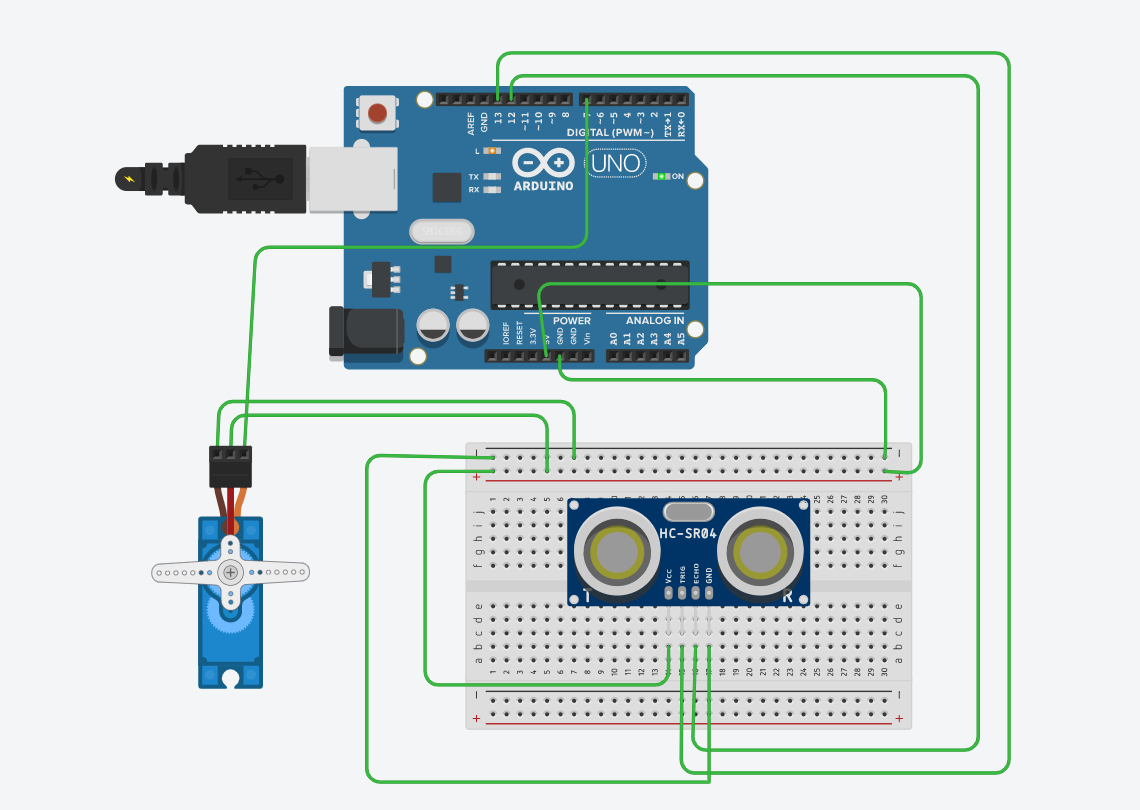
\includegraphics[width=.95\textwidth]{Screenshot_on_2023-05-01_at_23-47-24.png}
	\caption{Circuit Diagram}
\end{figure}

\section{Circuit Diagram}
\begin{figure}[H]
	\centering
	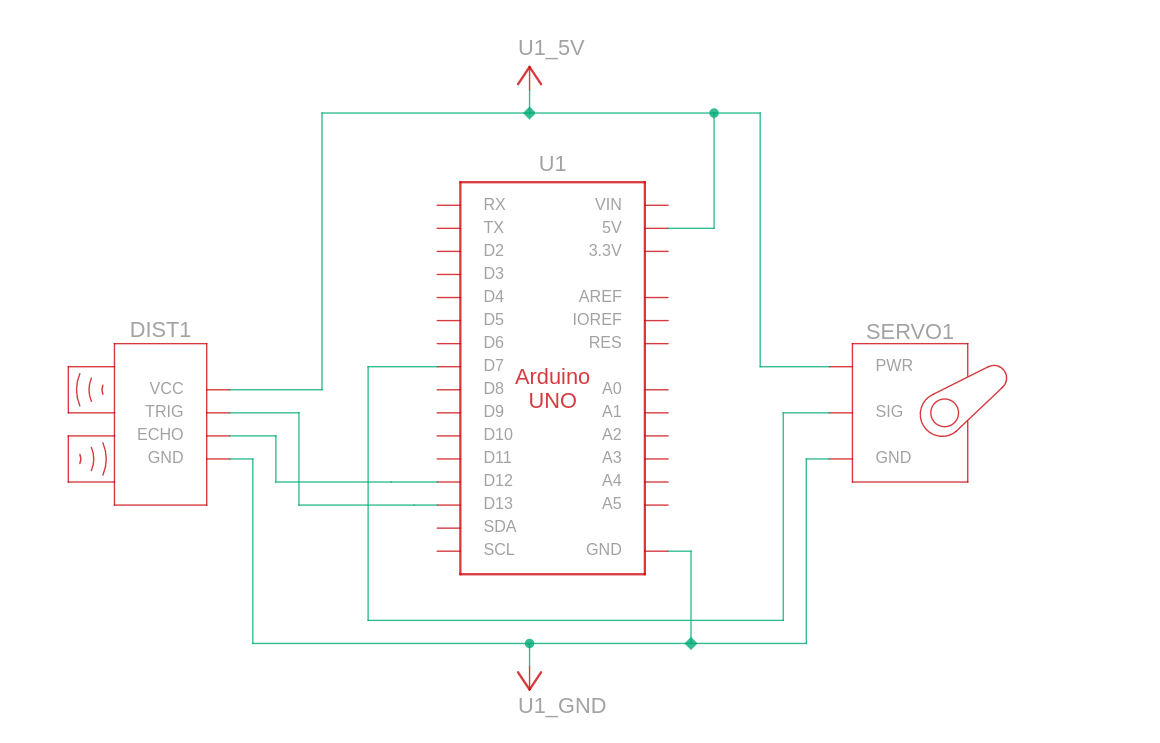
\includegraphics[width=.95\textwidth]{Screenshot_on_2023-05-01_at_23-52-00.png}
	\caption{Circuit Diagram}
\end{figure}


\section{Code}
\begin{lstlisting}[language=C++]
	#include<Servo.h>
	Servo srv;
	#define maxdistance 100
	void setup()
	{
	  Serial.begin(9600);
	  pinMode(13, OUTPUT);
	  pinMode(12, INPUT);
	  srv.attach(7);
	
	}
	
	void loop()
	{
	 
	  digitalWrite(13, LOW);
	  delay(1000); // Wait for 1000 millisecond(s)
	  digitalWrite(13, HIGH);
	  delay(1000); // Wait for 1000 millisecond(s)
	  digitalWrite(13, LOW);
	  int d=pulseIn(12,HIGH);
	  d=d/29/2;
	  Serial.println(d);
	  if(d<=maxdistance)
	  {
		srv.write(90);
		delay(1000);
	  }
	  else
	  {
		delay(1000);
		srv.write(0);
	  }
		
	}
\end{lstlisting}
\section{Conclusion}
Thus, we have successfully controlled the servo motor using the ultrasonic sensor and Arduino Uno.
\clearpage

\section{FAQ}

\begin{enumerate}
	\item Arduino Uno R3 (Code: U1)
	      \begin{itemize}
		      \item Type: Microcontroller board
		      \item Digital pins: 14
		      \item Analog input pins: 6
		      \item Operating voltage: 5V
		      \item Input voltage (recommended): 7-12V
		      \item Input voltage (limits): 6-20V
		      \item Flash memory: 32 KB (ATmega328P microcontroller)
		      \item SRAM: 2 KB (ATmega328P microcontroller)
		      \item EEPROM: 1 KB (ATmega328P microcontroller)
		      \item Clock speed: 16 MHz (ATmega328P microcontroller)
	      \end{itemize}
	\item Servo Motor (Code: M1)
	      \begin{itemize}
		      \item Type: DC motor with a built-in gear and feedback mechanism
		      \item Operating voltage: 4.8V to 6V
		      \item Stall torque: 1.8 to 12 kg-cm
		      \item Rotation angle: 0° to 180°
		      \item Control signal: Pulse width modulation (PWM)
		      \item Signal frequency: 50 Hz
	      \end{itemize}

\end{enumerate}

\end{document}